\chapter{Implementation and Performance Analysis}
In the previous section, we described the system's general architecture and the modules required to implement the tracking system. In this chapter, we will explain how the different parts are connected, and we will explain the implementation of the system.\\
The tracking system designed in this project uses Arduino module and the ُSIM 808, including the GSM and GPS antennas, for tracking. The core of this project is the Arduino microcontroller. The geographical location of object is received using a GPS antenna, and then this information is sent to the webserver using GSM technology. A web application has been developed to view and track an object on a map. This application consists of two parts: Front-end and Back-end. The front-end part has developed using Angular framework, and the Back-end part has developed using Express framework.\\
Initially, the SIM 808 module is initialized to get the location from the satellite. The initial settings of this device are done using AT commands. By connecting the GPS antenna, this module will be able to receive location coordinates from the satellite. Then the settings related to the GPRS network are done.\\
In fiqure 3.1 How to connect different modules in the tracking system is shown:\\
\begin{figure}[!h]
	\centerline{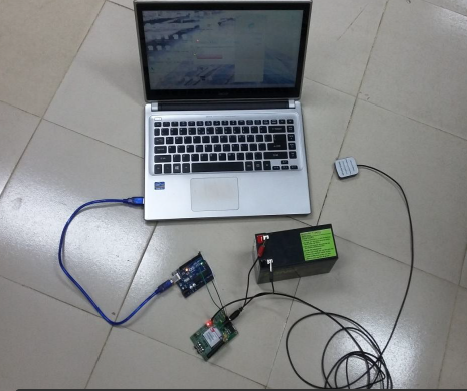
\includegraphics[width=.7\textwidth]{design-system}}
	\caption{Designed Tracking System}
\end{figure}\\
\section{Evaluate Tracking system performance}
As mentioned, the hardware part of our system consists of four modules, SIM 808, GSM receiver, GPS receiver, and Arduino microcontroller. This section will explain the implementation of the designed system, how to connect the various components and the implemented code.
\subsection{Circuit performance evaluation}
Before dealing with the modules and how to connect them, it is necessary to observe the system microcontroller performance and processing information in the flowchart. The overall performance of the system was described in the previous section. Now we have a flowchart about the implemented algorithm, and we can have a better understanding of the workflow in the hardware circuit designed and the code written for it.\\
The following diagram shows the general process of the implemented code on the Arduino.
\begin{figure}[h!]
	\centering
	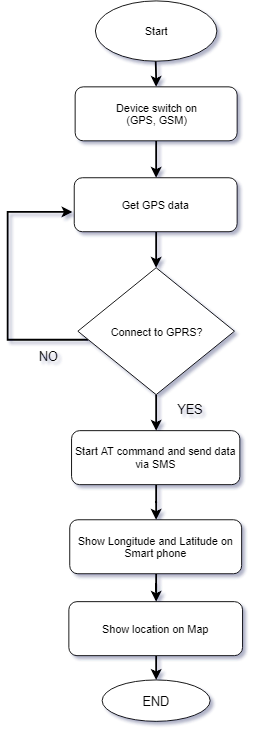
\includegraphics[width=.4\textwidth]{tracking-flowchart}
	\caption{Performance of implemented code on Arduino \cite{3}}
\end{figure}
\newpage
Firstly, for testing the system, the GPS antenna is connected to the SIM 808 module to receive the object's location (latitude and longitude) from the satellite. For doing this, the Arduino IDE software is used to program the code written on the Arduino board.\\
\newpage
The flowchart 3.3 shows how GPS works:\\
\begin{figure}[!h]
	\centerline{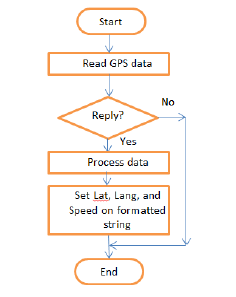
\includegraphics[width=.6\textwidth]{gps-flowchart}}
	\caption{Read Information diagram \cite{8}}
\end{figure}

For sending the object's location to the user via the GSM network, SIM 808 module and the Arduino microcontroller connected to it are used. For connecting 808 SIM module to the GSM network, we use AT commands to program and control it.\\
\newpage
The flowchart 3.4 shows how GSM works:\\
\begin{figure}[!h]
	\centerline{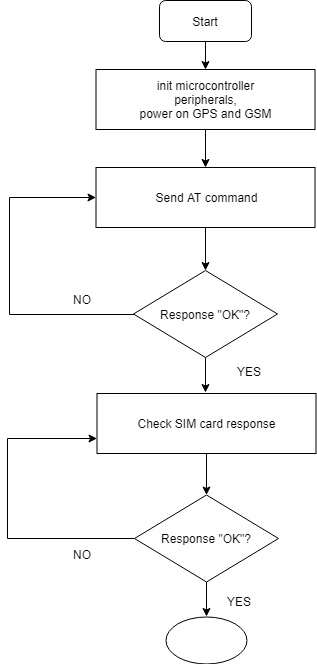
\includegraphics[width=.6\textwidth]{gsm-flowchart}}
	\caption{GSM \cite{8}}
\end{figure}
\newpage`
\begin{figure}[!h]
	\centerline{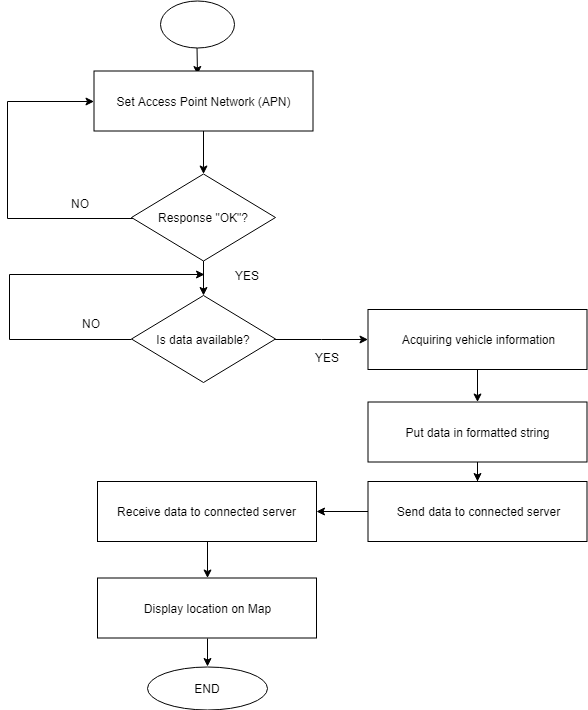
\includegraphics[width=.9\textwidth]{continue-gsm}}
	\caption{GSM \cite{8}}
\end{figure}
\newpage
\section{Circuit Architecture evaluation}

In this section, we explain the hardware part of the proposed system. As mentioned in the previous sections, using GPS antenna connected to the SIM 808 module, location information is received from the satellite every two minutes and then sent to the server via the GSM network.\\
In the following figure, you can see how to connect SIM 808 module to the Arduino.
\begin{figure}[!h]
	\centerline{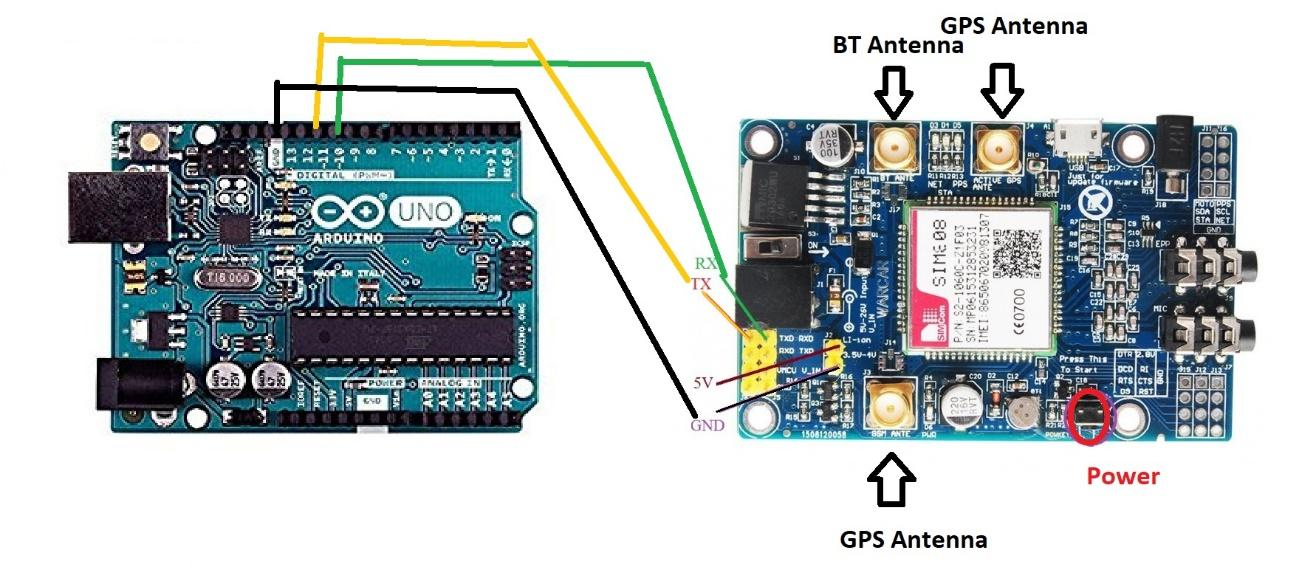
\includegraphics[width=.8\textwidth]{sim808-arduino}}
	\caption{SIM 808 - Arduino}
\end{figure}\\

The 808 SIM module is connected to the Arduino using a serial interface; it has two TX and RX pins connected to the 10 and 11 Arduino digital pins, respectively. The ground pin of this module is also connected to the ground connection base of the Arduino board. We supply the required voltage of the 808 SIM module through a 9-volt output adapter.
\section{Application}
In the Back-end, a web service with RESTful architecture has been developed, which stores the received data in the database, and the web application receives and displays this information.

REST is a web service architecture that uses HTTP to exchange information between two systems. The basic idea of this architecture is to use HTTP to establish information between machines instead of using complex mechanisms to connect devices.

In this section, we first describe the structure of the database and how to communicate with it. Finally, we explain the written web application that shows the path of the object on the map.
\subsubsection{Database}
We have used Mango database to store information and manage the server. Mango DB is a NOSQL database that runs on various operating systems, including Windows and Macintosh Linux. It also supports most programming languages. Mango DB provides high performance, accessibility, scalability, fast repeatability, and automatic sharing.
Due to the NOSQL structure, Mango DB only stores and searches data, thus significantly increasing data acquisition and storage speed.

The database received information from the hardware side. Then we store this information, including latitude, longitude, time, and date.

\subsection{Present Information}
\subsubsection{Web Application}
A web application has been developed to display the information stored in the database. The front-end of this web application is implemented using the Angular framework, and we use Google Maps to show the route.\\
This web application is available at the following address: http:// 103.216.62.79

Server-side processes were implemented using the Express framework. The server-side code works in such a way that as soon as new data is received from the hardware side, this data is stored in the Mango database. The hardware sends an HTTP request to the server each time it sends new data to the server: /api/device/add/

